\documentclass[tikz,border=2pt]{standalone}
\usepackage{amsmath,amssymb}
\usepackage{tikz}
\usetikzlibrary{arrows.meta}

\begin{document}
% For any two real numbers exactly one of a<b, a=b, a>b holds: on the line, a is to the left of b,
% on top of b, or to the right of b.
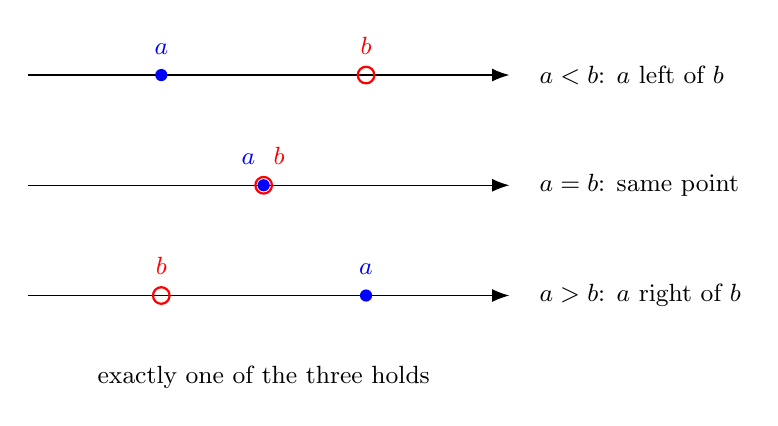
\begin{tikzpicture}[x=1.3cm, every node/.style={font=\small}]
	\foreach \y/\pa/\pb/\lab in {1.4/1/3/{$a<b$: $a$ left of $b$}, 0/2/2/{$a=b$: same point}, -1.4/3/1/{$a>b$: $a$ right of $b$}} {
		\draw[-{Latex[length=2.2mm]}] (-0.3,\y) -- (4.4,\y);
		\fill[blue] (\pa,\y) circle (2.2pt);
		\draw[red, thick] (\pb,\y) circle (3pt);
		\node[anchor=west] at (4.6,\y) {\lab};
	}
	\node[blue, above=4pt] at (1,1.4) {$a$}; \node[red, above=4pt] at (3,1.4) {$b$};
	\node[blue, above=4pt] at (1.85,0) {$a$}; \node[red, above=4pt] at (2.15,0) {$b$};
	\node[red, above=4pt] at (1,-1.4) {$b$}; \node[blue, above=4pt] at (3,-1.4) {$a$};
	\node[below=22pt, align=center] at (2,-1.4) {exactly one of the three holds};
\end{tikzpicture}
\end{document}
